\documentclass{article}
\usepackage[italian]{babel}
\usepackage{microtype}
\usepackage[utf8]{inputenc}
\usepackage{hyperref}
\usepackage[italian]{cleveref}
\usepackage[sort, round]{natbib}
\usepackage{graphicx}
\usepackage[margin=2cm]{geometry}
\usepackage[table,xcdraw]{xcolor}
\title{Q-learning su FPGA}
\date{\today}
\author{Davide Ragazzini \and Kevin Michael Frick}

\begin{document}
\maketitle

\section{Introduzione}
Il \emph{reinforcement learning} è una branca dell'apprendimento macchina orientato allo sviluppo di algoritmi in grado di massimizzare la \emph{funzione di reward} totale in un \emph{processo decisionale Markoviano}, ovvero un \emph{ambiente} che espone uno \emph{stato} e delle \emph{azioni}. 
Questi algoritmi tentano di stimare una funzione $q(s, a)$ che restituisce la massima reward ottenibile scegliendo l'azione $a$ quando l'ambiente è nello stato $s$. 
% algoritmi on-policy e off-policy
Gli algoritmi più recenti si servono di reti neurali, che si possono dimostrare essere in grado di approssimare funzioni qualunque, ma esistono algoritmi detti \emph{classici} come Q-learning \citep{watkins_learning_1989}. 
Q-learning è un algoritmo on-policy che si serve di una matrice stato-azione $Q$ (da cui il nome) la cui cella corrispondente alla riga $s$ e colonna $a$ contiene una stima della reward totale per lo stato $s$ l'azione $a$. 
A ogni periodo $t$ l'agente seleziona un'azione $a_t$, osserva la reward $r_t$ e transiziona allo stato $s_{t + 1}$ funzione dello stato corrente $s_t$ e dell'azione $a_t$. 

A ogni iterazione dell'algoritmo la matrice $Q$ viene aggiornata secondo la seguente espressione

$$
Q'(s_t, a_t) \leftarrow Q(s_t, a_t) + \alpha (r_t + \gamma \max_a Q(s_{t+1}, a) - Q(s_t, a))
$$

dove $\gamma$ è detto \emph{discount factor} e $\alpha$ è detta \emph{learning rate}. 

\section{Implementazione}
L'algoritmo è stato implementato servendosi di Vitis HLS, Vivado e Vitis nella versione 2020.2. 
I test sono stati eseguiti su una ZedBoard, una development board per la FPGA Zynq-7000 All Programmable SoC XC7Z020-CLG484-1, con periodo di clock impostato a $T = 10 \textrm{ns}$.
È stato scelto come caso di test il task \emph{CartPole} ovvero il bilanciamento del pendolo invertito. 
Le variabili di stato di questo task sono:

\begin{itemize}
\item $x$, la posizione del carrello
\item $\dot{x}$, la velocità del carrello
\item $\theta$, l'angolo formato dall'asta del pendolo e dall'asse orizzontale
\item $\dot{\theta}$, la velocità angolare dell'estremità superiore del pendolo
\end{itemize}

Le azioni disponibili sono solo due: spostare il carrello di un intervallo $\delta x$ a destra o a sinistra, ovvero $A = \{x \leftarrow x + \delta x, x \leftarrow x - \delta x\}$. 

\subsection{Vitis HLS}
Il cuore del progetto è una IP che implementa Q-learning, realizzata nel linguaggio C++ e tradotta in VHDL mediante il software Vitis HLS. 

La top-function dell'IP generata è \texttt{learn()}, che riceve in input un \texttt{hls::stream} di numeri casuali a 32 bit, utilizzati per inizializzare la matrice $Q$, decidere tra exploration ed exploitation con probabilità $\epsilon$ di exploration e scegliere casualmente un'azione in caso di exploration. 
Si è scelto di disaccoppiare la generazione di numeri casuali dalla top-function di apprendimento, inserendo una direttiva che richieda a Vitis HLS di tradurre questo argomento in una porta AXI-Stream sulla IP generata. 
Gli altri argomenti della top-function sono la porta di uscita \texttt{running}, che verrà poi collegata ai LED della ZedBoard per fornire informazioni sullo stato dell'IP, la porta di ingresso \texttt{id} contenente un identificatore dell'agente, cablato a 0, e le due porte di I/O \texttt{failures} e \texttt{q\_table} che verrano mappate alla DRAM del PS mediante il protocollo AXI4. 
Il valore restituito dalla top function è comunicato al PS mediante il protocollo AXI4 Lite. 
L'azione scelta e lo stato attuale sono passati alla \texttt{get\_state()} che restituisce lo stato risultante. 
Lo spazio degli stati è continuo con dimensione 4, ma viene mappato a un insieme limitato di 162 possibili stati, le righe della matrice $Q$, mediante la funzione \texttt{discretize()}. 

Fattorizzando la funzione di stato futuro e la discretizzazione delle azioni e avendo cura di definire in maniera appropriata costanti che rappresentino la dimensione dello spazio degli stati e delle azioni, la top-function può rimanere inalterata al variare dei task ed è possibile adattare l'IP a un nuovo task scrivendo solamente queste due funzioni. 

La convergenza è definita come l'apprendimento di una policy in grado di bilanciare il pendolo per almeno 195 periodi in media mobile sulle ultime 50 epoche. 

Nella \cref{table:synthesis} vengono riportati i risultati della sintesi VHDL della IP.

\begin{table}[h!]
\label{table:synthesis}
\end{table}
\subsection{Vivado}
Si è scelto di usare \href{https://github.com/wfedorko/Mersenne-Twister-HLS}{una IP open source} che implementa l'algoritmo Mersenne Twister per generare numeri casuali. 

Lo schema a blocchi definito su Vivado è rappresentato in \cref{fig:bd}.
\begin{figure}[h!]

\centering


\includegraphics[width=0.5\textwidth]{bd.png}
\label{fig:bd}
\end{figure}

\subsection{Vitis}
Il PS viene utilizzato per inizializzare la Q-table scrivendo sulla DRAM, avviare l'IP e leggere il valore restituito dalla top function. 

\subsection{Stima dell'occupazione della memoria}
Un singolo elemento di una matrice $Q$ è un numero in virgola mobile a 32 bit (4 byte).
La ZedBoard utilizzata per la valutazione dispone di 512 MiB di DRAM.
Senza considerare l'\emph{overhead} introdotto dal modulo di generazione di numeri casuali, sarebbe quindi possibile sulla carta memorizzare una matrice $Q$ con più di 100 milioni di elementi. 

\section{Prestazioni}
L'algoritmo è stato testato passando in input 1000 \emph{seed} diversi per il generatore di numeri casuali che inizializza la $Q$-table e determina sperimentazione o exploitation.
I risultati ottenuti in media tra i 1000 seed sono riportati nella \cref{table:perf} e visualizzati nella \cref{fig:perf}.

\begin{figure}[h!]

\centering


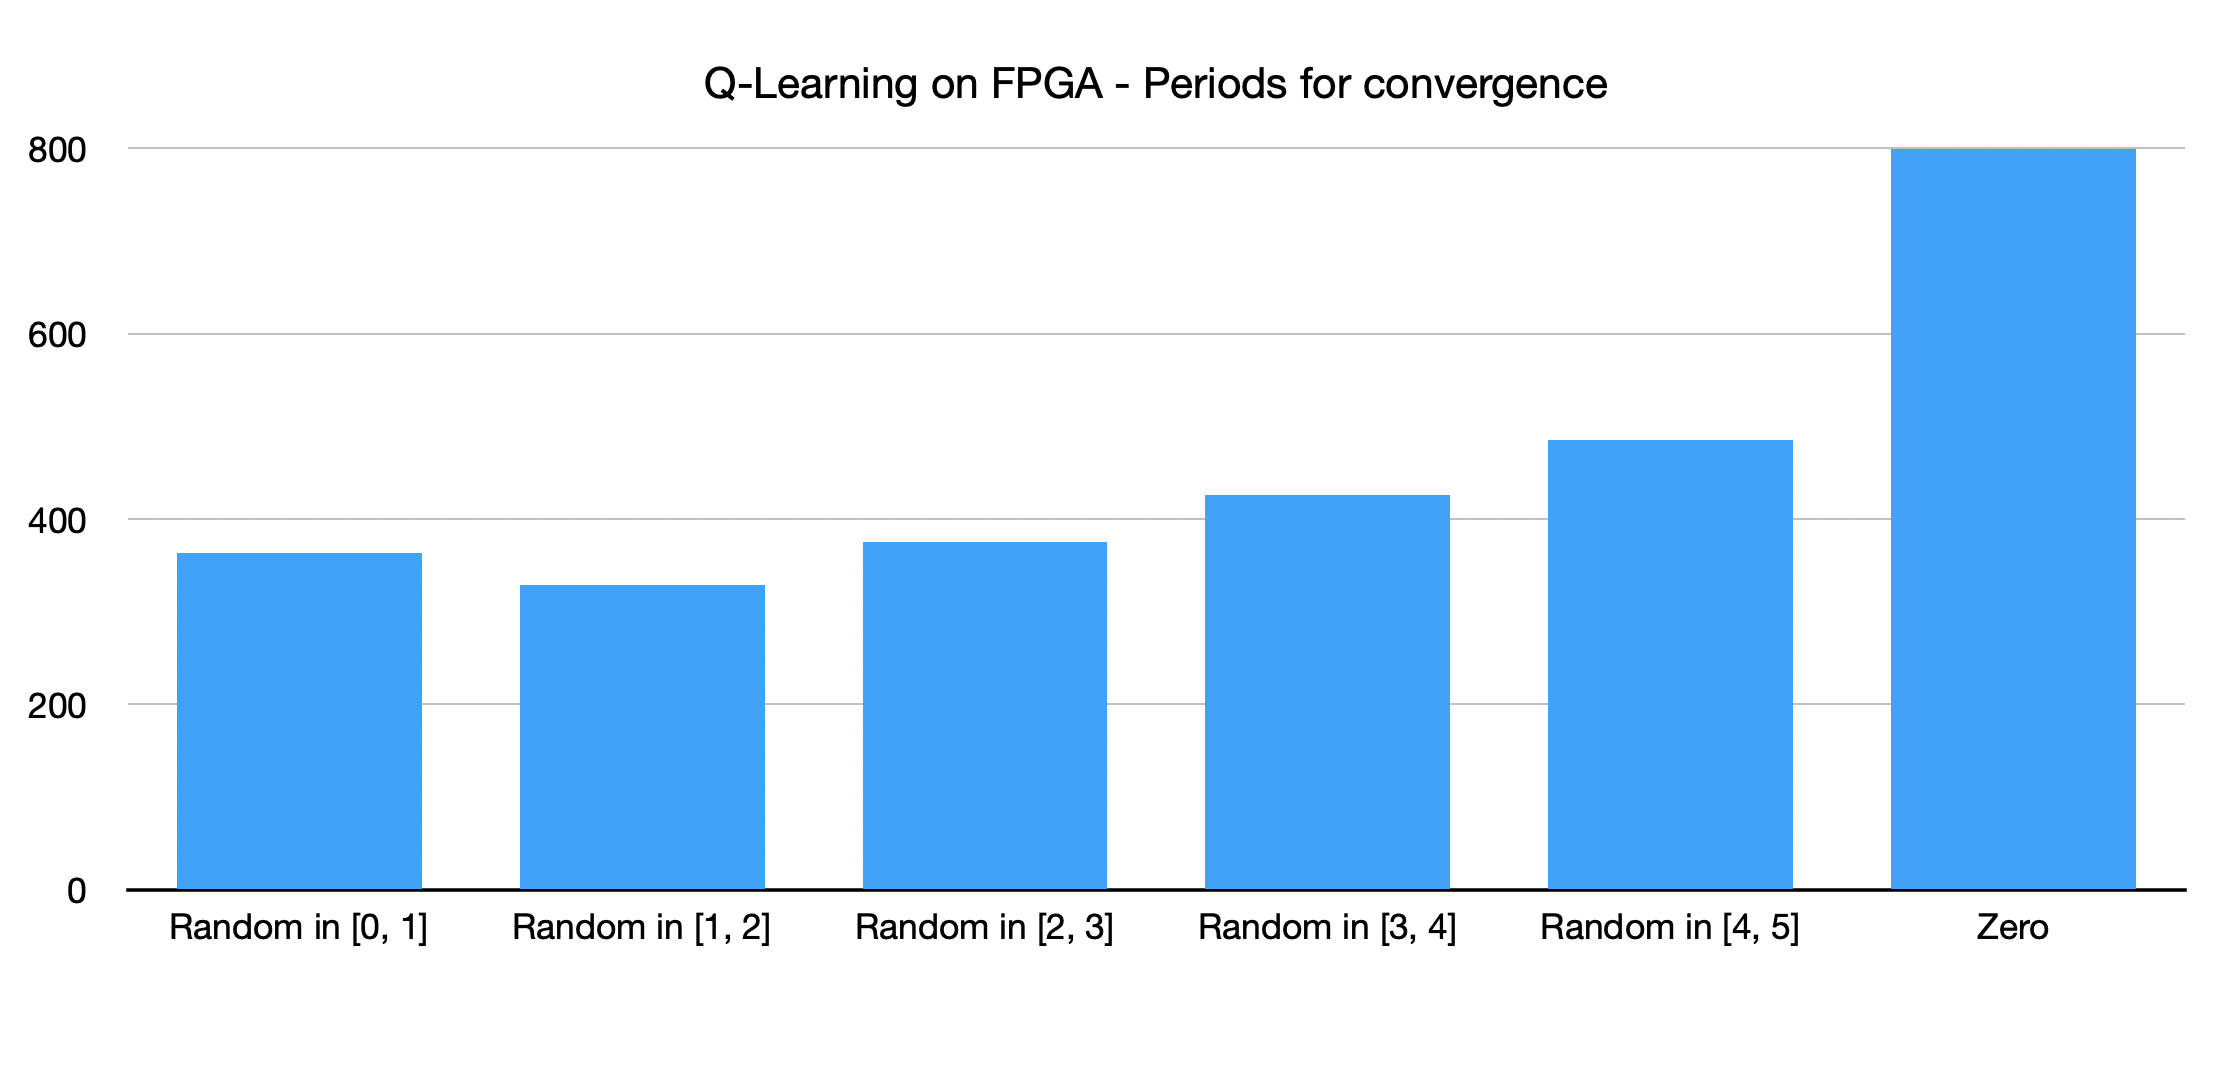
\includegraphics[width=0.5\textwidth]{perf.png}
\label{fig:perf}
\end{figure}

\begin{table}[h!]

\centering


\begin{tabular}{|
	>{\columncolor[HTML]{EFEFEF}}l |l|}
	\hline
	& \cellcolor[HTML]{EFEFEF}\textbf{Periodi per la convergenza (s)} \\ \hline
	\textbf{Inizializzazione casuale}             &                                                                 \\ \hline
	\textbf{Inizializzazione casuale ottimistica} &                                                                 \\ \hline
	\textbf{Inizializzazione a 0}                 &                                                                 \\ \hline
	\textbf{}                                     &                                                                 \\ \hline
	\end{tabular}
	\label{table:perf}
	\end{table}
	\section{Evoluzioni future}
	Il codice HLS è stato impostato in modo da permettere l'implementazione di apprendimento multiagente \citep{kretchmar_parallel_2002} mediante la condivisione degli array \texttt{failures} e \texttt{q\_table} tra più moduli uguali nella PL.
	L'implementazione e il testing di questo tipo di apprendimento saranno oggetto dell'attività progettuale di Sistemi Digitali M.
	\bibliographystyle{plainnat}
	\nocite{*}
	\bibliography{main}
	\end{document}

